\documentclass{article}
\usepackage[utf8]{inputenc}
\usepackage{graphicx}

\graphicspath{{./}}

\title{Visualizing Pokemon Stats}
\author{Paul White}
\date{March 2022}

\begin{document}

\maketitle

\section{Data Cleaning}
The main issue with data pulled from Serebii is that there are columns whose values on the site are images, and some, like secondary Abilities being nonexistent for many Pokemon. Fortunately, the data set only uses fully evolved Pokemon. Additionally, there are several Pokemon that are used twice, because this set includes Mega Evolutions as well as other forms; I got rid of these so as to use only base forms. To do this, I sorted by Base Stat Total, then used the distinct function to get rid of subsequent entries of the same Pokedex number, which is the same Pokemon, but under a different form, such as Deoxys' stat specialized forms, Mega Evolutions, or regional variants (such as Alolan Muk). The goal is to use only base forms over time, not the stronger forms added later on. All of the numeric variables also had to be converted to numeric data types.

I also created a new column called StatRange, which was calculated by subtracting the Pokemon's lowest base stat from its highest. The idea here was to test if Pokemon have become more min/maxed over time (that is, if the range of their highest and lowest stat has increased).

\section{Base Stat Totals by Dex No.}

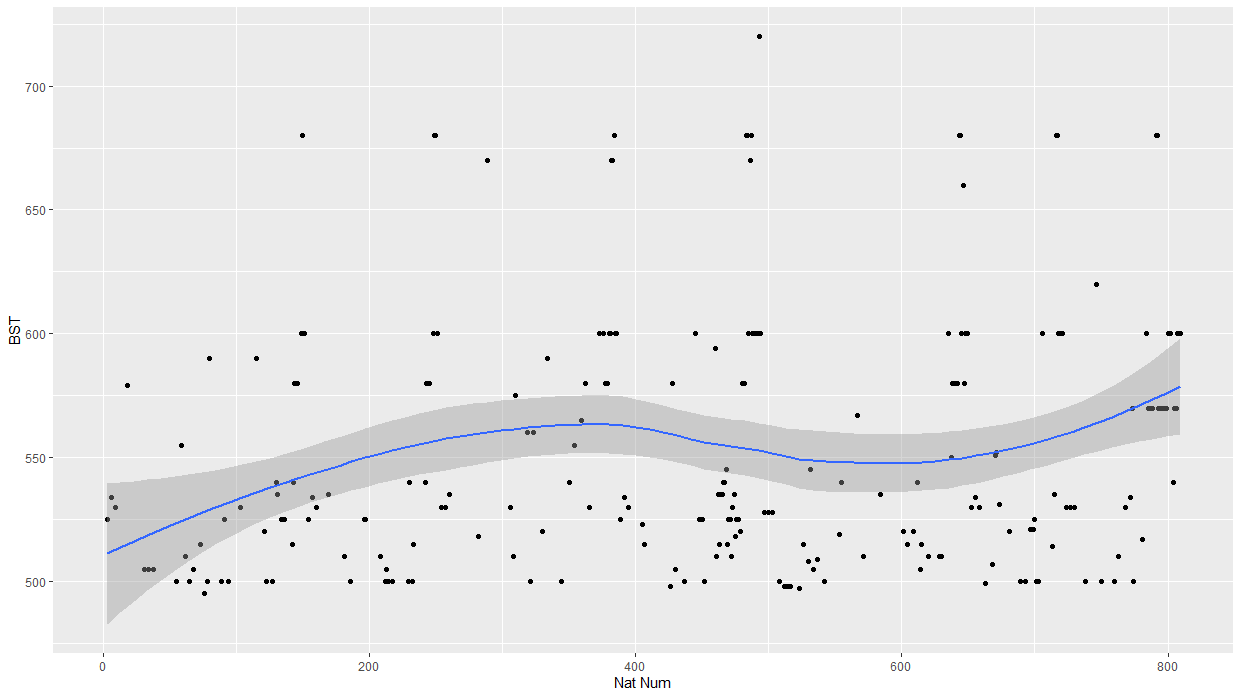
\includegraphics[scale = .4]{PS6a_White.png}
This is a graph of base stat totals as Pokedex number increases. As one can see, there is something of an increase in total stats over time. There is likely a periodic effect due to the fact that every new set of Pokemon tends to end with Legendary Pokemon, which are typically much stronger than other Pokemon.

\section{Stat Range by Dex No.}

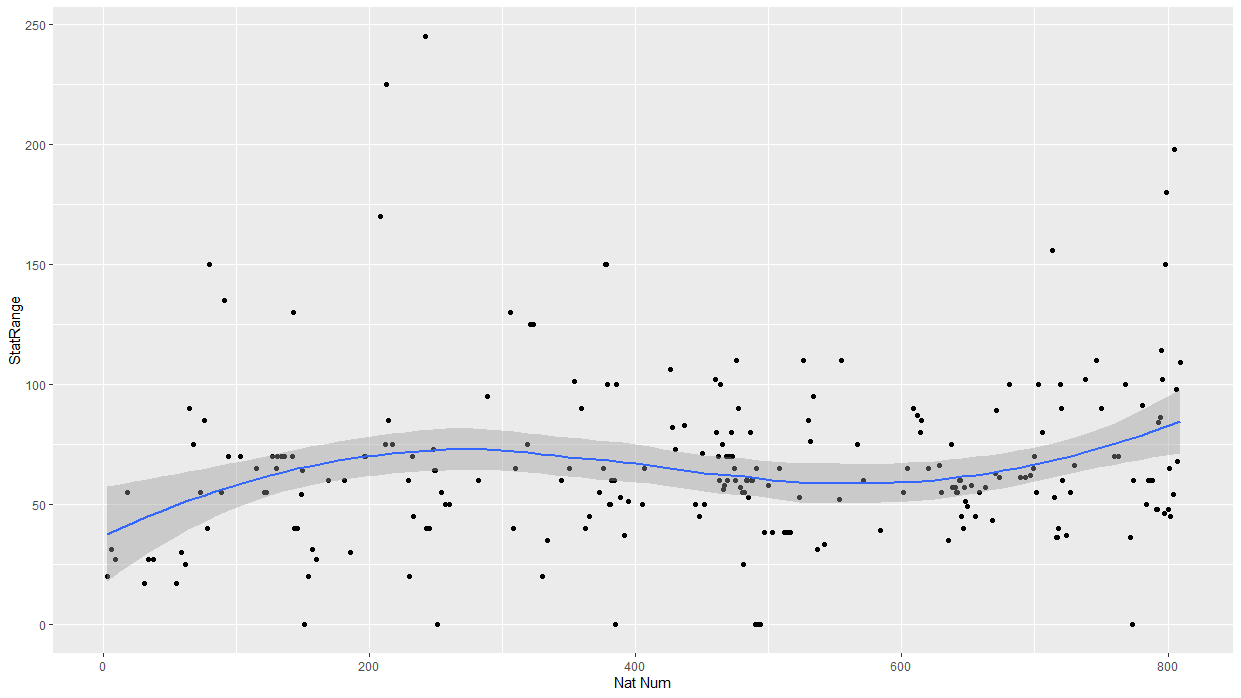
\includegraphics[scale = .4]{PS6b_White.png}
This shows that there is an overall increase in the range between the highest and lowest stat of each Pokemon. This likely has to do with the increasing focus on competitive play within Pokemon.

\section{Stat Range by Base Stat Total}

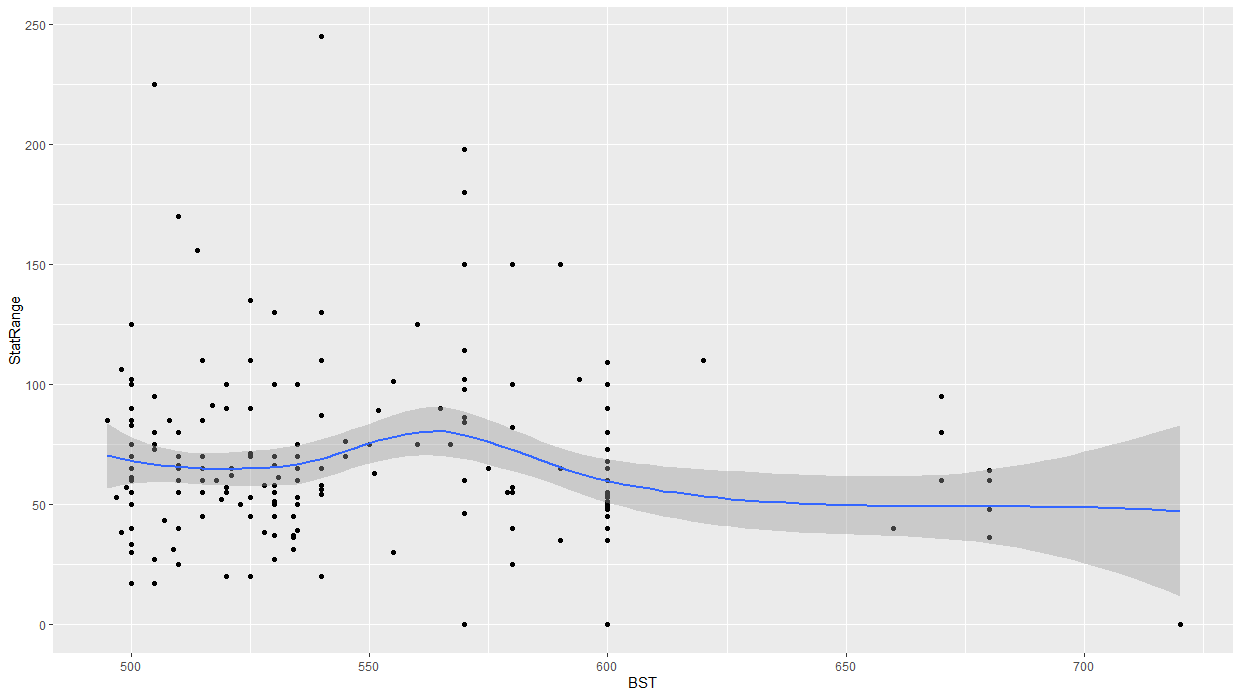
\includegraphics[scale = .4]{PS6c_White.png}
This was to see if Pokemon become more min/maxed as they become stronger. It would appear that there are Pokemon with greater than 500 total stats and less than 600 that show much greater stat range, on average. However, past that range, there is less range, likely because Legendaries tend to have all-around balanced stat spreads.

\end{document}
